
%%%%%%%%%%%%%%%%%%%%%%%%%%%%%%%%%%%%%%%%%%%%%%%%%%%%%%%%%%
%%
%% MARK: Title & Data
%%
%%%%%%%%%%%%%%%%%%%%%%%%%%%%%%%%%%%%%%%%%%%%%%%%%%%%%%%%%%

\chapter*{\S B22. The Parasymplectic Space of \hbox{Geodesics Trajectories}}
\setcounter{footnote}{0}

%%%%%%%%%%%%%%%%%%%%%%%%%%%%%%%%%%%%%%%%%%%%%%%%%%%%%%%%%%
%%
%% MARK: Abstract
%%
%%%%%%%%%%%%%%%%%%%%%%%%%%%%%%%%%%%%%%%%%%%%%%%%%%%%%%%%%%

\begin{abstract}
  We describe the parasymplectic structure on the space of geodesics trajectories of any Riemannian manifold.
\end{abstract}

%%%%%%%%%%%%%%%%%%%%%%%%%%%%%%%%%%%%%%%%%%%%%%%%%%%%%%%%%%
%%
%% MARK: The Space Of Geodesics Of A Riemmanian Manifold
%%
%%%%%%%%%%%%%%%%%%%%%%%%%%%%%%%%%%%%%%%%%%%%%%%%%%%%%%%%%%

We consider a Hausdorff and second countable manifold $M$ equipped with a Riemannian metric $g$.
The construction of the space of geodesic trajectories is described in §\ref{On-geodesics}.
Quotient spaces are equipped with quotient diffeology.
Let $ UM$ be the unit tangent bundle
$$
  UM = \{y = (x,u) \mid x \in M \text{ and } u \in T_x(M) \text{ with } g(u,u) = 1 \}.
  $$
The space of (oriented) geodesic trajectories $\Geod(M)$ is defined as the space of characteristics of the presymplectic form $d\lambda$ defined on $UM$,
where $\lambda$ is the Cartan form
$$
  \lambda (\delta y) = g(u, \delta x),
  $$
for all $\delta y \in T_y(UM)$.
Its differential $d\lambda$ is given by
$$
  d\lambda(\delta y, \delta'y) = g(\hat \delta u,\delta'x) - g(\hat \delta' u,\delta x),
  $$
where $\hat \delta u$ is defined by its coordinates in the charts:
$$
  \hat \delta u^\mu = \delta u^\mu + \Gamma^\mu_{\nu\rho}u^\nu\delta x^\rho.
  $$
The $\Gamma^\mu_{\nu\rho}$ are the Christoffel symbols.
We have seen that $\delta y \in \ker(d\lambda)$ if and only if:
$$
  \hat\delta u = 0 \text{ and } \delta x \propto u.
  $$
Thus,
there is only one vector $\xi \in T_y(UM)$ such that:
$$
  \xi \in \ker(d\lambda) \text{ and } \lambda(\xi) = 1.
  $$
It is defined by
$$
  \xi = \delta y \text{ with } \delta x = u \text{ and } \hat\delta u = 0.
  $$%
This vector $\xi$ is called \emph{Reeb vector}.

\textbf{Definition.} {\it A \emph{contact form} on a manifold $Y$ is any $1$-form $\lambda$ such that
$$
\ker(\lambda) \cap \ker(d\lambda) = \{0\},
$$%
and the \emph{Reeb vector field} is defined by
$$
  \xi \in \ker(d\lambda) \text{ and } \lambda(\xi) = 1.
  $$}%

We accept th following proposition:

\textbf{Proposition.} {\it Two point $y$ and $y'$ are on the same characteristic of $d\lambda$,
that is,
on an integral curve of the distribution $y \mapsto \ker(d\lambda)$,
if and only if there is a real number $s$ such that:
$$
  e^{s\xi}(y) = y',
  $$
where $e^{s\xi}$ denotes the local flow $e^{t\xi}$ of the Reeb vector $\xi$.
}

The Reeb vector field on $UM$ generates what is called the \emph{geodesic flow}.
We have then the following theorem:

\textbf{Theorem.} {\it Let $Y$ be a manifold,
Hausdorff and second countable,
equipped with a contact form $\lambda$.
Then,
there always exists on the space $\cS$ of charateristics of $d\lambda$ a parasymplectic form $\omega$ such that
$$
\Class^*(\omega) = d\lambda,
$$
where $\Class : Y \to \cS = Y/\ker(d\lambda)$ is the projection.\,%
When $\cS$ is a manifold then $\omega$ is symplectic,
but in any case $\omega$ still is a closed $2$-form on $\cS$.
This is an example of \emph{symplectic reduction} with singularities similar to the one in Ex.~\ref{quasiprojective-space-reduction}.
Moreover,
if $Y$ has dimension $2n-1$ (contact manifolds are odd dimensional) then $\cS$ has dimension $2n-2$.
}

\begin{proof}
  We recall that the Reeb vector field of a contact form generates by integration a local $1$-parameter of automorphisms of $\lambda$.
  Indeed,
  thanks to the Cartan formula one has first the vanishing Lie derivative:
  $$
    \cL_\xi(\lambda) = [d\lambda](\xi) + d[\lambda(\xi)] = 0 + 0.
    $$
  Thus,
  the local flow $e^{t\xi}$ of the vector $\xi$ preserves $\lambda$\,:
  $$
    {e^{t\xi}}^*(\lambda) = \lambda.
    $$
  To prove that the form $d\lambda$ passes to the quotient $X$,
  we shall apply the criterion \cite[\textsection 6.38]{PIZ13}.
  Let $P,P' \colon U \to Y$ be two plots in $Y$ such that $\pi \circ P = \pi \circ P'$.
  Let $r_0 \in U$,
  by hypothesis,
  $P(r_0)$ and $P'(r_0)$ belongs to the same characteristic.
  Then,
  there exists a real number $s$ such that $e^{s\xi}(P(r_0)) = P'(r_0)$.
  The local diffeomorphism $e^{s\xi}$ is defined on some neighbourhood of $P(r_0)$ and its inverse $e^{-s\xi}$,
  on some neighborhood of $P'(r_0)$.
  The composite $P'' = e^{-s\xi} \circ P'$ is then defined on some neighbourhood $\cO'$ of $r_0$ and satisfies:
  $\pi \circ P = \pi \circ P''$ and $P(r_0) = P''(r_0)$.
  Now,
  thanks to the \emph{flow box theorem},
  there exists a local diffeomorphism $\phi$ from a neighbourhood $\cO''$ of $P(r_0)$,
  that maps $\cO''$ to a product $W \times \cI'$,
  where $\cI'$ is some real interval,
  the vector field $\xi$ to $(0,1)$ and $e^{s\xi}$ to the translation $(w,t) \mapsto (w,t+s)$.
  We assume that $\phi(P(r_0)) = (0,0)$.
  The intersection $U' = (\phi \circ P)^{-1}(W \times \cI') \cap (\phi \circ P'')^{-1}(W \times \cI')$ is open and non empty since it contains $r_0$.
  We will restrict $P$ and $P'$ to $U'$.
  Consider now,
  $(\pi \circ \phi^{-1}) \restriction W \times \{0\}$,
  since our manifolds are assumed Hausdorff and second countable,
  the preimages in $W$ of characteristics are countable,
  and because $W$ is an Euclidean domain,
  they are (diffeologically) discrete \cite[Exercice 8]{PIZ13}.
  Therefore,
  restricting $P$ and $P''$ to a ball $\cB$ centered at $r_0$,
  $\pi \circ P = \pi \circ P''$ implies $\Proj_1 \circ \phi \circ P(r) = \Proj_1 \circ \phi \circ P''(r)$,
  for all $r \in \cB$.
  That is,
  $\phi \circ P(r) = (f(r), t(r))$ and $\phi \circ P''(r) = (f(r), t''(r))$,
  where the maps involved are smooth.
  Hence,
  there a smooth real map $r \mapsto s(r) = t''(r) - t(r)$ such that $P''(r) = e^{s(r)\xi}(P(r))$,
  for all $r \in \cB$.
  Let us write simply $\underline{s(r)}_Y = e^{s(r)\xi}$,
  then $P''(r) = \underline{s(r)}_Y(P(r))$,
  and $s \mapsto \underline{s}_Y$ is a local additive action on $Y$.
  Remember now that because $\xi \in \ker(d\lambda)$ and $\lambda(\xi) = 1$ the Lie derivative vanishes: $\cL_\xi(\lambda)= 0$,
  and then $(e^{s\xi})^*(\lambda) = \lambda$,
  or $\underline{s}_Y^*(\lambda) = \lambda$.
  Thus,
  thanks to \cite[\textsection 8.37]{PIZ13},
  \begin{align*}
    \lambda(P'')_r & = \lambda\big(r \mapsto \underline{s(r)}_Y(P(r))\big)_r \\
    & = [\underline{s(r)}_Y^*(\lambda)](P)_r + [\Rm(P(r))^*(\lambda)](s)_r  \\
    & = \lambda(P)_r + ds_r,
  \end{align*}
  where we denoted $\Rm(y)(s) = \underline{s}_Y(y)$.
  Hence,
  $d\lambda(P'') = d\lambda(P)$ on the ball $\cB$,
  and then on all $U$.
  Therefore,
  according to the criterion \cite[\textsection 6.38]{PIZ13},
  there exists a $2$-form $\omega$ on $X$ such that $d\lambda = \pi^*(\omega)$.
  And $\omega$ is closed since $\pi^*(d\omega) = 0$ \cite[\textsection 6.39]{PIZ13}.
  
  As for the dimension of the quotient,
  the diffeology of $\cS = Y/\ker(d\lambda)$ is generated by the transversal of the flow of the Reeb vector which are $2n-2$ plots.
  When one can choose such transversal that cuts each orbit of the geodesic flow in one and only one point,
  then they are local diffeomorphisms with the quotient $\cS$,
  and $\cS$ is a manifold.
  On that manifold the $2$-form $\omega$ is non degenerate,
  therefore symplectic.
  Otherwise,
  and this is the most general case,
  one cannot find such transversal everywhere and the flow cuts some of them infinitely many times.
  It is what happens in particular on the $2$-torus for irrational geodesics.
\end{proof}

\textbf{Corollary.} {\it The space $\Geod(M)$ of geodesic trajectories,
equipped with the quotient diffeology of the unit tangent bundle $UM$ by the kernel of the differential $d\lambda$,
has dimension $2n-2$ and is parasymplectic for a closed $2$-form $\omega$ defined by $\Class^*(\omega) = d\lambda$.
When $\Geod(M)$ is a manifold then $\omega$ is symplectic.
}

\textbf{Definition.} {\it We shall call \emph{symplectically generated} any parasymplectic space that admits a generating family of plots where the pullback of the parasymplectic form is symplectic.}

Then,
the parasymplectic structure on the quotient space $\cS$ in the general case of a contact form,
and on $\Geod(M)$ in particular,
is symplectically generated.
Indeed,
the restrictions of $d\lambda$ on the transversals of the Reeb vector field is non-degenerate since $\ker(d\lambda) = \xi\RR$.
They give a generating family of plots on which the pullback of $\omega$ is symplectic.
This is why I decided to call \emph{symplectically generated} this kind of parasymplectic space.
That includes the spaces of geodesic trajectories as we just saw,
but also the cone orbifolds \cite[\textsection 9.32]{PIZ13} or Prato's toric quasifolds \cite{EP01}.

%\vfill\n
%\centerline{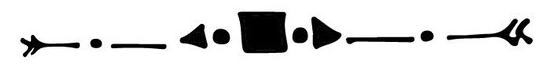
\includegraphics[width=.5\textwidth]{Figures/separator.png}}\n
